%%%%%%%% ICML 2024 EXAMPLE LATEX SUBMISSION FILE %%%%%%%%%%%%%%%%%

\documentclass{article}

% Recommended, but optional, packages for figures and better typesetting:
\usepackage{microtype}
\usepackage{graphicx}
\usepackage{multicol}
\usepackage{subfigure}
\usepackage{booktabs} % for professional tables
\usepackage{adjustbox}

% hyperref makes hyperlinks in the resulting PDF.
% If your build breaks (sometimes temporarily if a hyperlink spans a page)
% please comment out the following usepackage line and replace
% \usepackage{icml2024} with \usepackage[nohyperref]{icml2024} above.
\usepackage{hyperref}


% Attempt to make hyperref and algorithmic work together better:
\newcommand{\theHalgorithm}{\arabic{algorithm}}

% Use the following line for the initial blind version submitted for review:
\usepackage{icml2024}

% If accepted, instead use the following line for the camera-ready submission:
% \usepackage[accepted]{icml2024}

% For theorems and such
\usepackage{amsmath}
\usepackage{amssymb}
\usepackage{mathtools}
\usepackage{amsthm}
\usepackage{booktabs} % For professional looking tables
\usepackage{tabularx} % For tables with adjustable-width columns

% if you use cleveref..
\usepackage[capitalize,noabbrev]{cleveref}

%%%%%%%%%%%%%%%%%%%%%%%%%%%%%%%%
% THEOREMS
%%%%%%%%%%%%%%%%%%%%%%%%%%%%%%%%
\theoremstyle{plain}
\newtheorem{theorem}{Theorem}[section]
\newtheorem{proposition}[theorem]{Proposition}
\newtheorem{lemma}[theorem]{Lemma}
\newtheorem{corollary}[theorem]{Corollary}
\theoremstyle{definition}
\newtheorem{definition}[theorem]{Definition}
\newtheorem{assumption}[theorem]{Assumption}
\theoremstyle{remark}
\newtheorem{remark}[theorem]{Remark}

% Todonotes is useful during development; simply uncomment the next line
%    and comment out the line below the next line to turn off comments
%\usepackage[disable,textsize=tiny]{todonotes}
\usepackage[textsize=tiny]{todonotes}


% The \icmltitle you define below is probably too long as a header.
% Therefore, a short form for the running title is supplied here:
\icmltitlerunning{Enhancing Antibiotic Stewardship using a Natural Language Approach for Better Feature Representation}

\begin{document}

\twocolumn[
\icmltitle{Enhancing Antibiotic Stewardship using a Natural Language Approach for Better Feature Representation}

% It is OKAY to include author information, even for blind
% submissions: the style file will automatically remove it for you
% unless you've provided the [accepted] option to the icml2024
% package.

% List of affiliations: The first argument should be a (short)
% identifier you will use later to specify author affiliations
% Academic affiliations should list Department, University, City, Region, Country
% Industry affiliations should list Company, City, Region, Country

% You can specify symbols, otherwise they are numbered in order.
% Ideally, you should not use this facility. Affiliations will be numbered
% in order of appearance and this is the preferred way.
\icmlsetsymbol{equal}{*}

\begin{icmlauthorlist}
\icmlauthor{Simon A. Lee}{yyy}
\icmlauthor{Trevor Brokowski}{zzz,aaa}
\icmlauthor{Jeffrey N. Chiang}{yyy,comp}
%\icmlauthor{}{sch}
%\icmlauthor{}{sch}
\end{icmlauthorlist}

\icmlaffiliation{yyy}{Department of Computational Medicine, UCLA}
\icmlaffiliation{comp}{Department of Neurosurgery, UCLA}
\icmlaffiliation{zzz}{Yale School of Medicine}
\icmlaffiliation{aaa}{Biomedical Informatics \& Data Science, Yale University}

\icmlcorrespondingauthor{Simon A. Lee}{simonlee711@g.ucla.edu}
\icmlcorrespondingauthor{Jeffrey Chiang}{njchiang@g.ucla.edu}

% You may provide any keywords that you
% find helpful for describing your paper; these are used to populate
% the "keywords" metadata in the PDF but will not be shown in the document
\icmlkeywords{Machine Learning, ICML}

\vskip 0.3in
]

% this must go after the closing bracket ] following \twocolumn[ ...

% This command actually creates the footnote in the first column
% listing the affiliations and the copyright notice.
% The command takes one argument, which is text to display at the start of the footnote.
% The \icmlEqualContribution command is standard text for equal contribution.
% Remove it (just {}) if you do not need this facility.

%\printAffiliationsAndNotice{}  % leave blank if no need to mention equal contribution
\printAffiliationsAndNotice{\icmlEqualContribution} % otherwise use the standard text.

\begin{abstract}
The rapid emergence of antibiotic-resistant bacteria is recognized as a global healthcare crisis, undermining the efficacy of life-saving antibiotics. This crisis is driven by the improper and overuse of antibiotics, which escalates bacterial resistance. In response, this study explores the use of clinical decision support systems, enhanced through the integration of electronic health records (EHRs), to improve antibiotic stewardship. However, EHR systems present numerous data-level challenges, complicating the effective synthesis and utilization of data. In this work, we transform EHR data into a serialized textual representation and employ pretrained foundation models to demonstrate how this enhanced feature representation can aid in antibiotic susceptibility predictions. Our results suggest that this text representation, combined with foundation models, provides a valuable tool to increase interpretability and support antibiotic stewardship efforts.
\end{abstract}

\section{Introduction}

The Centers for Disease Control and Prevention (CDC) has declared the rapid emergence of resistant bacteria a global healthcare crisis, threatening the efficacy of antibiotics that have saved millions of lives \citep{ventola2015antibiotic, golkar2014bacteriophage, gould2013new, sengupta2013multifaceted, nature2013antibiotic, lushniak2014antibiotic}. This crisis is primarily driven by the mishandling and overuse of these antibiotics, which leads to bacteria developing resistance through repetitive exposure \cite{viswanathan2014off, read2014antibiotic}. 
% Additionally, the pharmaceutical industry has faced criticism for its lack of new drug development, largely attributed to stringent regulatory policies \cite{piddock2012crisis}. 
These resistant bacteria impose significant clinical and financial burdens on healthcare systems, as well as on patients and their families worldwide \cite{bartlett2013seven}.

Clinical decision support systems hold substantial potential to assist healthcare providers in adhering to antibiotic stewardship practices. This potential is largely facilitated by electronic health record (EHR) software, which allows for the seamless integration of patient health histories in digital form \cite{evans2016electronic, cowie2017electronic, hoerbst2010electronic}. The integration with EHRs enables the use of continuously updated and deployed machine learning models for clinical decision-making. However, EHR data in its raw form presents numerous challenges, such as data ingestion and feature representation \cite{wu2010prediction}.

In this work, we present a methodology that converts EHR data into a serialized text form called pseudo-notes to predict antibiotic susceptibility. This conversion from tabular to text format facilitates the creation of interpretable data inputs for pretrained foundation models, known for their rich feature representation. Our primary objective is to develop a predictive model that incorporates this representation strategy in conjunction with foundation models. This approach aims to enhance decision support systems and accurately identify the most suitable antibiotics for patients, thereby offering a data-driven solution to combat antibiotic resistance.

\section{Related Works}

\paragraph{Medical Representation Learning}

Medical representation learning on Electronic Health Records (EHRs) has emerged as a critical area in healthcare research, focusing on transforming complex medical data for enhanced clinical decision-making. Initially, this involved extensive feature engineering to convert raw EHR data into formats suitable for traditional machine learning models \cite{tang2020democratizing, ferrao2016preprocessing}. However, this approach can be labor-intensive and varies significantly across research groups due to the lack of a standard protocol. 

Recently, the focus has shifted to advanced foundation models that learn to represent medical data by analyzing extensive text corpora, including clinical notes, medical literature, and records. These models, primarily based on the BERT architecture, generate rich, contextual latent representations of patient histories, significantly reducing the manual effort in feature engineering  \cite{rasmy2021med,liu2021med,alsentzer2019publicly,lee2020biobert}. Moreover, new techniques have been developed to incorporate the longitudinal nature of EHR data, leveraging a patients progression to predict outcomes \cite{steinberg2023motor, wornow2024ehrshot, pang2021cehr, li2022hi}.

\paragraph{Clinical Decision Support}

Machine learning enhances clinical decision support systems by analyzing vast datasets to provide evidence-based recommendations that improve patient care outcomes \cite{sutton2020overview}. Since the accessibility to EHR systems, there have been numerous such use cases in predicting diseases \cite{liu2018deep, cheng2016risk}, and various other patient outcomes \cite{lee2024emergency, suter1994predicting, churpek2014using} across all institutions within the healthcare system. Furthermore, the integration of predictive models into clinical workflows enables researchers to preemptively manage chronic conditions and mitigate potential health crises before they escalate \cite{li2020electronic, goldstein2017opportunities, hohman2023leveraging}. By continuously learning from new data, these systems evolve to provide more accurate assessments and recommendations, which support ongoing improvements in medical practices and patient management strategies. However, much work remains to be done on addressing the generalization and biases prevalent in many of these predictive algorithms \cite{goetz2024generalization, agniel2018biases}.

\section{Methods}
\paragraph{EHR} Electronic Health Records are digital versions of a patient’s medical history, maintained over time by healthcare providers. These records are valuable but consist of heterogeneous tabular datasets organized into separate tables such as diagnostics, demographics, and medication, presenting numerous challenges for researchers.

The primary challenge with EHRs is the heterogeneous nature of the data, which includes numerical, categorical, and free-text formats that are difficult to integrate and convert into machine-readable formats. Furthermore, categorical data fields often contain a large number of classes, potentially distorting their original representation. For instance, employing feature engineering techniques such as dummy coding for categorical variables can introduce collinearity, increase dimensionality, and result in sparse data representations. These modifications can complicate simple table readouts and require more memory capacity for statistical models to function effectively.

\paragraph{Pseudo-notes: Clinical Notes Generation from Tabular Data} Recent research has introduced a methodology for serializing tabular data into text using text templates \cite{hegselmann2023tabllm}. This approach significantly enhances our work by enabling uniform representation of all data in the EHR as human-readable and interpretable text, rather than as a collection of merged tables. Moreover, it creates an interface to use foundation models pre-trained on large text corpora, facilitating rich feature representation. In our work, we use a mapping function \( f: T \rightarrow S \) that turns individual tables into serialized text, where \( T \) stands for individual tables and \( S \) for serialized text. For each patient, we convert each of their $N$ tables—which cover different aspects like diagnostics, medications, and vitals—into text segments. These segments are then joined to create a single, detailed paragraph per patient. This method combines all pertinent patient information from various sources into one unified narrative, effectively transforming the data structure into \( S = \bigcup_{i=1}^{N} f(T_i) \), where \( T_i \) is the ith table row concerning the patient.

\paragraph{Data Source and Inclusion Criteria}

\begin{figure*}[t!]
\vskip -0.1in
\begin{center}
\centerline{\includegraphics[width=6.5in]{auroc.png}}
% \centerline{\includegraphics[width=\textwidth]{icml2024/auprc.png}}
\caption{Area under the Receiver Operating Characteristic (AUROC) curves for each antibiotic classification shows that, despite the nuances, BioMegatron performs the best.}
\label{auroc}
\end{center}
\vskip -0.1in
\end{figure*}

We sourced data from the Medical Information Mart for Intensive Care IV (MIMIC-IV) and MIMIC-IV Emergency Department (ED) databases \cite{johnson2020mimic, johnson2023mimic}. This study focused on ED patients presumed to have staph infections, selected based on specific inclusion criteria. Eligible participants included those with any microbiological culture testing positive for a staph-related organism, sourced from bodily fluids such as blood, urine, cerebral spinal fluid, pleural cavity, or joint fluid, accompanied by a prescribed antibiotic whose susceptibility was subsequently tested \cite{tong2015staphylococcus, kwiecinski2020staphylococcus}. From these criteria, we identified 5976 unique prescriptions in our database. Additionally, patients with multiple ED admissions that met the criteria were analyzed separately but were grouped within the same train/test divisions to prevent test set contamination. This cohort included 10 unique antibiotics, whose prevalences are shown in Table \ref{antibiotic-prevalence-table}. A demographic overview of our cohort is presented in Appendix Section \ref{demo}.

\begin{table}[h!]
\caption{Antibiotic Prevalence in MIMIC IV Cohort}
\label{antibiotic-prevalence-table}
\vskip 0.15in
\begin{center}
\begin{small}
\begin{sc}
\begin{adjustbox}{width=\columnwidth}
\begin{tabular}{lccc}
\toprule
Antibiotic & Train & Test & Total Prevalence (\%) \\
\midrule
Clindamycin & 2645 & 624 & \textbf{54.69\%} \\
Daptomycin & 1815 & 425 & \textbf{37.51\%} \\
Erythromycin & 2626 & 639 & \textbf{54.59\%} \\
Gentamicin & 4549 & 1127 & \textbf{94.89\%} \\
Levofloxacin & 2866 & 715 & \textbf{60.00\%} \\
Oxacillin & 2702 & 667 & \textbf{56.32\%} \\
Rifampin & 1929 & 459 & \textbf{39.96\%} \\
Tetracycline & 3747 & 909 & \textbf{76.57\%} \\
Trimethoprim/sul & 3671 & 908 & \textbf{71.66\%} \\
Vancomycin & 2529 & 611 & \textbf{52.53\%} \\
\bottomrule
\end{tabular}
\end{adjustbox}
\end{sc}
\end{small}
\end{center}
\vskip -0.1in
\end{table}

To motivate our experimental setup, we examine the information available about a patient at their time of arrival in the emergency department. To predict antibiotic use, we utilize six clinical modalities from the MIMIC ED Database. These EHR modalities include arrival and triage information, medication reconciliation (medrecon), diagnostic codes (ICD-9/10), vital signs, and Pyxis data. All these data points are linked to antibiotic labels from the MIMIC database using a patient ID, visit, and Hospital Admission ID (Hadm\_id), allowing us to accurately identify the patients and their tests in which certain antibiotics were effective.

\paragraph{Experiments}
In this work, we benchmark different representation strategies of EHR to identify the most effective method for predicting antibiotic susceptibility. We approach this problem as a multilabel binary classification, where we train the same base model (Light Gradient Boosted Machines) using various representation startegies of the input. These representations include: raw tabular data; EHR-shot \cite{wornow2024ehrshot}, a foundation model for tabular EHR; and three text-based representations: word2vec, a generic language model, and a medical language model, BioMegatron \cite{shin2020biomegatron}. Additionally, we conduct a clustering of our pseudonotes using the BERTopic algorithm \cite{grootendorst2022bertopic} to determine if these embeddings can naturally cluster patients. Identifying these clusters can provide insights into their potential performance in settings like zero-shot learning and provide insights into the decision making process.

\section{Results}

\begin{figure*}[h!]
\vskip 0.1in
\begin{center}
% \centerline{\includegraphics[width=\textwidth]{icml2024/auroc.png}}
\centerline{\includegraphics[width=6.5in]{auprc.png}}
\caption{Area under the Precision Recall Curve (AUPRC) curves for each antibiotic classification shows that, despite the nuances, BioMegatron performs the best.}
\label{auprc}
\end{center}
\vskip -0.1in
\end{figure*}

\paragraph{Antibiotic Susceptibility Prediction} In our analysis of antibiotic prediction, we measure the Area Under the Receiver Operating Characteristic curve (AUROC) and Area Under the Precision-Recall Curve (AUPRC). Additionally, we bootstrap 1,000 times to generate 95\% confidence intervals. Our AUROC and AUPRC results are displayed in Figures \ref{auroc} and \ref{auprc}. We also measure additional F1 scores and Matthews correlation coefficients, with a whole table readout which are included in the appendix.

\paragraph{Clustering Experiment} In our clustering experiments, we aim to identify clusters using the BERTopic algorithm. By identifying clusters based on embeddings, we believe this approach can form the basis for zero-shot applications across various clinical tasks. Additionally, finding similar embeddings could provide insights into decision-making processes in these black-box models. We showcase the similarity matrix of our patient clusters in Figure \ref{sim}.

\section{Discussion}

\paragraph{Clinical Notes with Foundation Models Provide the best representation and interpretability}

\begin{figure}[t!]
\begin{center}
% \centerline{\includegraphics[width=\textwidth]{icml2024/auroc.png}}
\centerline{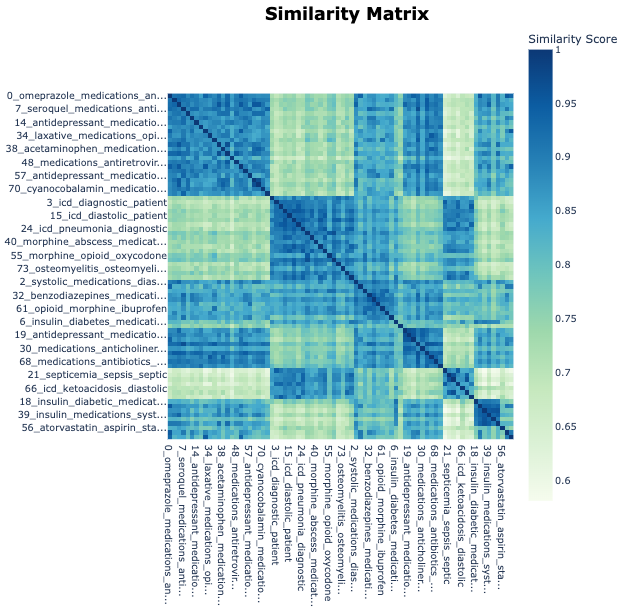
\includegraphics[width=3in]{similarity.png}}
\caption{Identifying clusters from our patient embeddings is indicated by the squares forming along the diagonal of our similarity matrix.}
\label{sim}
\end{center}
\vspace{-1cm}
\end{figure}

From Figures \ref{auroc} and \ref{auprc}, we observe that the foundation models operating on our pseudo-notes method provide the best overall performance across most of the antibiotics. While a generic foundation model and EHR-shot excel with some antibiotics, the clinical foundation model consistently shows superior performance across both AUROC and AUPRC metrics.

Beyond enhanced predictive abilities, an advantage of our pseudo-notes method over EHR foundation models and tabular representations is its interpretability. Compared to the specific structuring required by EHR-shot, our method offers a simpler and more effective interface to understand the data that is being modeled which can improve the trust between AI and healthcare professionals.

\paragraph{Interoperability}

Another advantage of pseudo-notes over EHR foundation models is their interoperability with proprietary healthcare systems. Our method offers a straightforward interface for converting any EHR tabular data from tables to text. Our conversion also facilitates the use of off-the-shelf open-source foundation models. As improved models are continually developed, this data format provides an easy interface to adapt and swap the backbone for improved representation of our clinical text. Additionally, EHR foundation models do not operate on non-OMOP vocabularies, which limits its effectiveness on datasets like MIMIC-IV that utilize these specialized vocabularies.
% \paragraph{An Easy Interface for EHR Representation}

% One advantage of our clinical notes generation method, compared to approaches like EHR-shot, is its straightforward conversion of any information from the EHR into interpretable clinical text. Although our research initially focused on the Emergency Department, this methodology can encode the remaining clinical tables found in the MIMIC-IV database and is versatile enough to predict any downstream tasks defined within the EHR. We prefer this approach because it enables the use of off-the-shelf foundation models from platforms like Hugging Face, which are well-suited for processing these clinical notes inputs. We also prefer this simple methodology because it allows for interoperability with other healthcare systems which is a current limiation in existing foundation models made for EHR. For example, methods like EHR-shot rely on hardcoded rules to determine which clinical information is embedded, are incompatible with non-OMOP vocabularies, require extensive preparation to generate a single embedding, and do not support proprietary datasets from many institutions that may require similar analyses. Additionally, models operating on raw tabular data, TF-IDF, and Bag of Words are considered outdated and less effective especially when trying to synthesize EHR data.

\paragraph{Patient Similarity}
One final advantage of our pseudo-notes is illustrated in Figure \ref{sim}, which demonstrates the capability to perform a similarity search on our patient embeddings. From this analysis, we identified clusters related to sepsis, diabetes, stomach acid issues, anxiety, painkillers, respiratory conditions, and antidepressants. This opens up potential use cases for this data representation strategy to be used in zero-shot learning studies and offers insights into decision-making processes based on the embeddings. Further research is needed to explore both of these areas.

\section{Conclusion}

In this work, we introduced a methodology called pseudo-notes, which converts EHR tabular data into text to achieve an optimal representation strategy. We discovered that pseudo-notes outperformed various representation strategies and remains a highly flexible framework, compatible with the ongoing development of foundation model backbones, which could further enhance its performance. Additionally, we found that pseudo-notes can identify patient clusters within the EHR, opening up promising avenues for future studies in zero-shot learning and model interpretation.

From an application perspective, we demonstrated how a straightforward data transformation has emerged as an easy interface for making EHR data synergized before integrating it into machine learning models. We think that this strategy could be a better way to work with EHR data for future research and help build trust due to its interpretability. Particularly in this study, we illustrated its potential by identifying suitable antibiotics for patients arriving at the ED, where timely and accurate decisions are critical. We as a group have highlighted the importance of improving antibiotic stewardship and showcase the impact of data-driven strategies in addressing pressing healthcare challenges.

\subsection*{Impact Statement}
% positive - it offers an interface between modern AI (LLMs) and healthcare
% negative - it does not directly address the potential biases in LLMs, and therefore could potentially introduce existing issues with LLMs into healthcare applications. More work is needed on this front before it's ready for prime time

The goal of this work is to advance the field of Machine Learning in Healthcare, and thus presents a novel potential interface between modern NLP (Foundation models) and clinical data. 

% \section{Electronic Submission}
% \label{submission}

% Submission to ICML 2024 will be entirely electronic, via a web site
% (not email). Information about the submission process and \LaTeX\ templates
% are available on the conference web site at:
% \begin{center}
% \textbf{\texttt{http://icml.cc/}}
% \end{center}

% The guidelines below will be enforced for initial submissions and
% camera-ready copies. Here is a brief summary:
% \begin{itemize}
% \item Submissions must be in PDF\@. 
% \item \textbf{New to this year}: If your paper has appendices, submit the appendix together with the main body and the references \textbf{as a single file}. Reviewers will not look for appendices as a separate PDF file. So if you submit such an extra file, reviewers will very likely miss it.
% \item Page limit: The main body of the paper has to be fitted to 8 pages, excluding references and appendices; the space for the latter two is not limited. For the final version of the paper, authors can add one extra page to the main body.
% \item \textbf{Do not include author information or acknowledgements} in your
%     initial submission.
% \item Your paper should be in \textbf{10 point Times font}.
% \item Make sure your PDF file only uses Type-1 fonts.
% \item Place figure captions \emph{under} the figure (and omit titles from inside
%     the graphic file itself). Place table captions \emph{over} the table.
% \item References must include page numbers whenever possible and be as complete
%     as possible. Place multiple citations in chronological order.
% \item Do not alter the style template; in particular, do not compress the paper
%     format by reducing the vertical spaces.
% \item Keep your abstract brief and self-contained, one paragraph and roughly
%     4--6 sentences. Gross violations will require correction at the
%     camera-ready phase. The title should have content words capitalized.
% \end{itemize}

% \subsection{Submitting Papers}

% \textbf{Paper Deadline:} The deadline for paper submission that is
% advertised on the conference website is strict. If your full,
% anonymized, submission does not reach us on time, it will not be
% considered for publication. 

% \textbf{Anonymous Submission:} ICML uses double-blind review: no identifying
% author information may appear on the title page or in the paper
% itself. \cref{author info} gives further details.

% \textbf{Simultaneous Submission:} ICML will not accept any paper which,
% at the time of submission, is under review for another conference or
% has already been published. This policy also applies to papers that
% overlap substantially in technical content with conference papers
% under review or previously published. ICML submissions must not be
% submitted to other conferences and journals during ICML's review
% period.
% %Authors may submit to ICML substantially different versions of journal papers
% %that are currently under review by the journal, but not yet accepted
% %at the time of submission.
% Informal publications, such as technical
% reports or papers in workshop proceedings which do not appear in
% print, do not fall under these restrictions.

% \medskip

% Authors must provide their manuscripts in \textbf{PDF} format.
% Furthermore, please make sure that files contain only embedded Type-1 fonts
% (e.g.,~using the program \texttt{pdffonts} in linux or using
% File/DocumentProperties/Fonts in Acrobat). Other fonts (like Type-3)
% might come from graphics files imported into the document.

% Authors using \textbf{Word} must convert their document to PDF\@. Most
% of the latest versions of Word have the facility to do this
% automatically. Submissions will not be accepted in Word format or any
% format other than PDF\@. Really. We're not joking. Don't send Word.

% Those who use \textbf{\LaTeX} should avoid including Type-3 fonts.
% Those using \texttt{latex} and \texttt{dvips} may need the following
% two commands:

% {\footnotesize
% \begin{verbatim}
% dvips -Ppdf -tletter -G0 -o paper.ps paper.dvi
% ps2pdf paper.ps
% \end{verbatim}}
% It is a zero following the ``-G'', which tells dvips to use
% the config.pdf file. Newer \TeX\ distributions don't always need this
% option.

% Using \texttt{pdflatex} rather than \texttt{latex}, often gives better
% results. This program avoids the Type-3 font problem, and supports more
% advanced features in the \texttt{microtype} package.

% \textbf{Graphics files} should be a reasonable size, and included from
% an appropriate format. Use vector formats (.eps/.pdf) for plots,
% lossless bitmap formats (.png) for raster graphics with sharp lines, and
% jpeg for photo-like images.

% The style file uses the \texttt{hyperref} package to make clickable
% links in documents. If this causes problems for you, add
% \texttt{nohyperref} as one of the options to the \texttt{icml2024}
% usepackage statement.


% \subsection{Submitting Final Camera-Ready Copy}

% The final versions of papers accepted for publication should follow the
% same format and naming convention as initial submissions, except that
% author information (names and affiliations) should be given. See
% \cref{final author} for formatting instructions.

% The footnote, ``Preliminary work. Under review by the International
% Conference on Machine Learning (ICML). Do not distribute.'' must be
% modified to ``\textit{Proceedings of the
% $\mathit{41}^{st}$ International Conference on Machine Learning},
% Vienna, Austria, PMLR 235, 2024.
% Copyright 2024 by the author(s).''

% For those using the \textbf{\LaTeX} style file, this change (and others) is
% handled automatically by simply changing
% $\mathtt{\backslash usepackage\{icml2024\}}$ to
% $$\mathtt{\backslash usepackage[accepted]\{icml2024\}}$$
% Authors using \textbf{Word} must edit the
% footnote on the first page of the document themselves.

% Camera-ready copies should have the title of the paper as running head
% on each page except the first one. The running title consists of a
% single line centered above a horizontal rule which is $1$~point thick.
% The running head should be centered, bold and in $9$~point type. The
% rule should be $10$~points above the main text. For those using the
% \textbf{\LaTeX} style file, the original title is automatically set as running
% head using the \texttt{fancyhdr} package which is included in the ICML
% 2024 style file package. In case that the original title exceeds the
% size restrictions, a shorter form can be supplied by using

% \verb|\icmltitlerunning{...}|

% just before $\mathtt{\backslash begin\{document\}}$.
% Authors using \textbf{Word} must edit the header of the document themselves.

% \section{Format of the Paper}

% All submissions must follow the specified format.

% \subsection{Dimensions}




% The text of the paper should be formatted in two columns, with an
% overall width of 6.75~inches, height of 9.0~inches, and 0.25~inches
% between the columns. The left margin should be 0.75~inches and the top
% margin 1.0~inch (2.54~cm). The right and bottom margins will depend on
% whether you print on US letter or A4 paper, but all final versions
% must be produced for US letter size.
% Do not write anything on the margins.

% The paper body should be set in 10~point type with a vertical spacing
% of 11~points. Please use Times typeface throughout the text.

% \subsection{Title}

% The paper title should be set in 14~point bold type and centered
% between two horizontal rules that are 1~point thick, with 1.0~inch
% between the top rule and the top edge of the page. Capitalize the
% first letter of content words and put the rest of the title in lower
% case.

% \subsection{Author Information for Submission}
% \label{author info}

% ICML uses double-blind review, so author information must not appear. If
% you are using \LaTeX\/ and the \texttt{icml2024.sty} file, use
% \verb+\icmlauthor{...}+ to specify authors and \verb+\icmlaffiliation{...}+ to specify affiliations. (Read the TeX code used to produce this document for an example usage.) The author information
% will not be printed unless \texttt{accepted} is passed as an argument to the
% style file.
% Submissions that include the author information will not
% be reviewed.

% \subsubsection{Self-Citations}

% If you are citing published papers for which you are an author, refer
% to yourself in the third person. In particular, do not use phrases
% that reveal your identity (e.g., ``in previous work \cite{langley00}, we
% have shown \ldots'').

% Do not anonymize citations in the reference section. The only exception are manuscripts that are
% not yet published (e.g., under submission). If you choose to refer to
% such unpublished manuscripts \cite{anonymous}, anonymized copies have
% to be submitted
% as Supplementary Material via OpenReview\@. However, keep in mind that an ICML
% paper should be self contained and should contain sufficient detail
% for the reviewers to evaluate the work. In particular, reviewers are
% not required to look at the Supplementary Material when writing their
% review (they are not required to look at more than the first $8$ pages of the submitted document).

% \subsubsection{Camera-Ready Author Information}
% \label{final author}

% If a paper is accepted, a final camera-ready copy must be prepared.
% %
% For camera-ready papers, author information should start 0.3~inches below the
% bottom rule surrounding the title. The authors' names should appear in 10~point
% bold type, in a row, separated by white space, and centered. Author names should
% not be broken across lines. Unbolded superscripted numbers, starting 1, should
% be used to refer to affiliations.

% Affiliations should be numbered in the order of appearance. A single footnote
% block of text should be used to list all the affiliations. (Academic
% affiliations should list Department, University, City, State/Region, Country.
% Similarly for industrial affiliations.)

% Each distinct affiliations should be listed once. If an author has multiple
% affiliations, multiple superscripts should be placed after the name, separated
% by thin spaces. If the authors would like to highlight equal contribution by
% multiple first authors, those authors should have an asterisk placed after their
% name in superscript, and the term ``\textsuperscript{*}Equal contribution"
% should be placed in the footnote block ahead of the list of affiliations. A
% list of corresponding authors and their emails (in the format Full Name
% \textless{}email@domain.com\textgreater{}) can follow the list of affiliations.
% Ideally only one or two names should be listed.

% A sample file with author names is included in the ICML2024 style file
% package. Turn on the \texttt{[accepted]} option to the stylefile to
% see the names rendered. All of the guidelines above are implemented
% by the \LaTeX\ style file.

% \subsection{Abstract}

% The paper abstract should begin in the left column, 0.4~inches below the final
% address. The heading `Abstract' should be centered, bold, and in 11~point type.
% The abstract body should use 10~point type, with a vertical spacing of
% 11~points, and should be indented 0.25~inches more than normal on left-hand and
% right-hand margins. Insert 0.4~inches of blank space after the body. Keep your
% abstract brief and self-contained, limiting it to one paragraph and roughly 4--6
% sentences. Gross violations will require correction at the camera-ready phase.

% \subsection{Partitioning the Text}

% You should organize your paper into sections and paragraphs to help
% readers place a structure on the material and understand its
% contributions.

% \subsubsection{Sections and Subsections}

% Section headings should be numbered, flush left, and set in 11~pt bold
% type with the content words capitalized. Leave 0.25~inches of space
% before the heading and 0.15~inches after the heading.

% Similarly, subsection headings should be numbered, flush left, and set
% in 10~pt bold type with the content words capitalized. Leave
% 0.2~inches of space before the heading and 0.13~inches afterward.

% Finally, subsubsection headings should be numbered, flush left, and
% set in 10~pt small caps with the content words capitalized. Leave
% 0.18~inches of space before the heading and 0.1~inches after the
% heading.

% Please use no more than three levels of headings.

% \subsubsection{Paragraphs and Footnotes}

% Within each section or subsection, you should further partition the
% paper into paragraphs. Do not indent the first line of a given
% paragraph, but insert a blank line between succeeding ones.

% You can use footnotes\footnote{Footnotes
% should be complete sentences.} to provide readers with additional
% information about a topic without interrupting the flow of the paper.
% Indicate footnotes with a number in the text where the point is most
% relevant. Place the footnote in 9~point type at the bottom of the
% column in which it appears. Precede the first footnote in a column
% with a horizontal rule of 0.8~inches.\footnote{Multiple footnotes can
% appear in each column, in the same order as they appear in the text,
% but spread them across columns and pages if possible.}

% \begin{figure}[ht]
% \vskip 0.2in
% \begin{center}
% \centerline{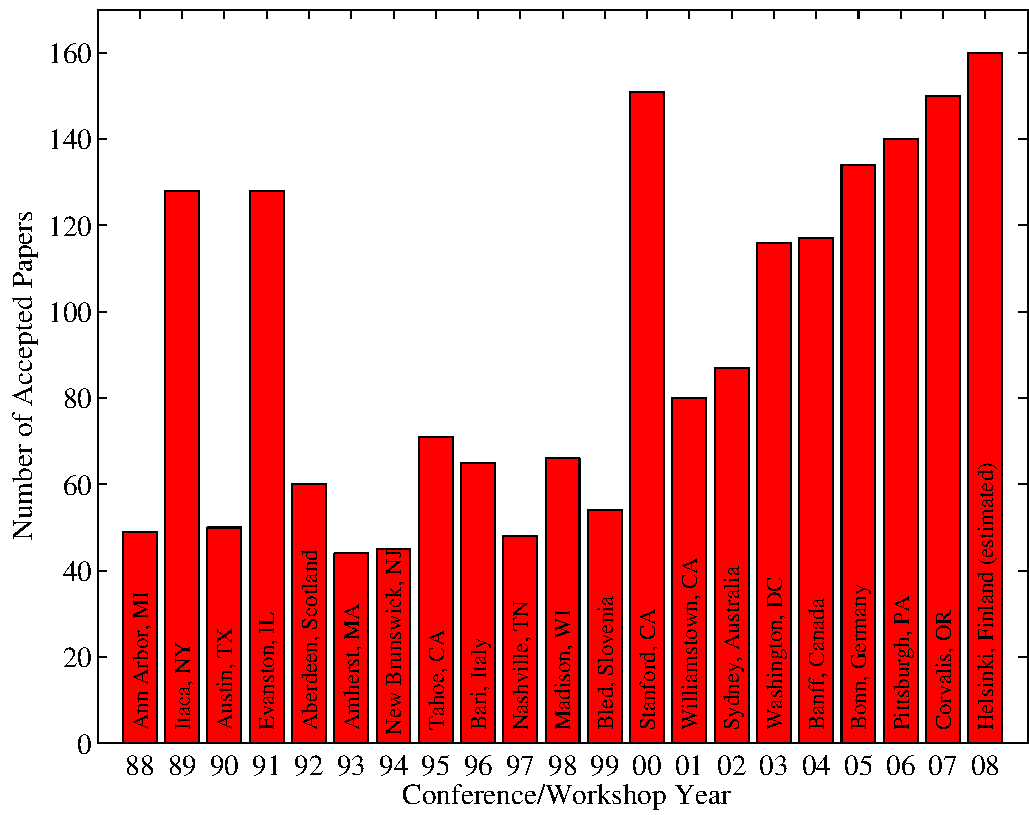
\includegraphics[width=\columnwidth]{icml_numpapers}}
% \caption{Historical locations and number of accepted papers for International
% Machine Learning Conferences (ICML 1993 -- ICML 2008) and International
% Workshops on Machine Learning (ML 1988 -- ML 1992). At the time this figure was
% produced, the number of accepted papers for ICML 2008 was unknown and instead
% estimated.}
% \label{icml-historical}
% \end{center}
% \vskip -0.2in
% \end{figure}

% \subsection{Figures}

% You may want to include figures in the paper to illustrate
% your approach and results. Such artwork should be centered,
% legible, and separated from the text. Lines should be dark and at
% least 0.5~points thick for purposes of reproduction, and text should
% not appear on a gray background.

% Label all distinct components of each figure. If the figure takes the
% form of a graph, then give a name for each axis and include a legend
% that briefly describes each curve. Do not include a title inside the
% figure; instead, the caption should serve this function.

% Number figures sequentially, placing the figure number and caption
% \emph{after} the graphics, with at least 0.1~inches of space before
% the caption and 0.1~inches after it, as in
% \cref{icml-historical}. The figure caption should be set in
% 9~point type and centered unless it runs two or more lines, in which
% case it should be flush left. You may float figures to the top or
% bottom of a column, and you may set wide figures across both columns
% (use the environment \texttt{figure*} in \LaTeX). Always place
% two-column figures at the top or bottom of the page.

% \subsection{Algorithms}

% If you are using \LaTeX, please use the ``algorithm'' and ``algorithmic''
% environments to format pseudocode. These require
% the corresponding stylefiles, algorithm.sty and
% algorithmic.sty, which are supplied with this package.
% \cref{alg:example} shows an example.

% \begin{algorithm}[tb]
%    \caption{Bubble Sort}
%    \label{alg:example}
% \begin{algorithmic}
%    \STATE {\bfseries Input:} data $x_i$, size $m$
%    \REPEAT
%    \STATE Initialize $noChange = true$.
%    \FOR{$i=1$ {\bfseries to} $m-1$}
%    \IF{$x_i > x_{i+1}$}
%    \STATE Swap $x_i$ and $x_{i+1}$
%    \STATE $noChange = false$
%    \ENDIF
%    \ENDFOR
%    \UNTIL{$noChange$ is $true$}
% \end{algorithmic}
% \end{algorithm}

% \subsection{Tables}

% You may also want to include tables that summarize material. Like
% figures, these should be centered, legible, and numbered consecutively.
% However, place the title \emph{above} the table with at least
% 0.1~inches of space before the title and the same after it, as in
% \cref{sample-table}. The table title should be set in 9~point
% type and centered unless it runs two or more lines, in which case it
% should be flush left.

% % Note use of \abovespace and \belowspace to get reasonable spacing
% % above and below tabular lines.

% \begin{table}[t]
% \caption{Classification accuracies for naive Bayes and flexible
% Bayes on various data sets.}
% \label{sample-table}
% \vskip 0.15in
% \begin{center}
% \begin{small}
% \begin{sc}
% \begin{tabular}{lcccr}
% \toprule
% Data set & Naive & Flexible & Better? \\
% \midrule
% Breast    & 95.9$\pm$ 0.2& 96.7$\pm$ 0.2& $\surd$ \\
% Cleveland & 83.3$\pm$ 0.6& 80.0$\pm$ 0.6& $\times$\\
% Glass2    & 61.9$\pm$ 1.4& 83.8$\pm$ 0.7& $\surd$ \\
% Credit    & 74.8$\pm$ 0.5& 78.3$\pm$ 0.6&         \\
% Horse     & 73.3$\pm$ 0.9& 69.7$\pm$ 1.0& $\times$\\
% Meta      & 67.1$\pm$ 0.6& 76.5$\pm$ 0.5& $\surd$ \\
% Pima      & 75.1$\pm$ 0.6& 73.9$\pm$ 0.5&         \\
% Vehicle   & 44.9$\pm$ 0.6& 61.5$\pm$ 0.4& $\surd$ \\
% \bottomrule
% \end{tabular}
% \end{sc}
% \end{small}
% \end{center}
% \vskip -0.1in
% \end{table}

% Tables contain textual material, whereas figures contain graphical material.
% Specify the contents of each row and column in the table's topmost
% row. Again, you may float tables to a column's top or bottom, and set
% wide tables across both columns. Place two-column tables at the
% top or bottom of the page.

% \subsection{Theorems and such}
% The preferred way is to number definitions, propositions, lemmas, etc. consecutively, within sections, as shown below.
% \begin{definition}
% \label{def:inj}
% A function $f:X \to Y$ is injective if for any $x,y\in X$ different, $f(x)\ne f(y)$.
% \end{definition}
% Using \cref{def:inj} we immediate get the following result:
% \begin{proposition}
% If $f$ is injective mapping a set $X$ to another set $Y$, 
% the cardinality of $Y$ is at least as large as that of $X$
% \end{proposition}
% \begin{proof} 
% Left as an exercise to the reader. 
% \end{proof}
% \cref{lem:usefullemma} stated next will prove to be useful.
% \begin{lemma}
% \label{lem:usefullemma}
% For any $f:X \to Y$ and $g:Y\to Z$ injective functions, $f \circ g$ is injective.
% \end{lemma}
% \begin{theorem}
% \label{thm:bigtheorem}
% If $f:X\to Y$ is bijective, the cardinality of $X$ and $Y$ are the same.
% \end{theorem}
% An easy corollary of \cref{thm:bigtheorem} is the following:
% \begin{corollary}
% If $f:X\to Y$ is bijective, 
% the cardinality of $X$ is at least as large as that of $Y$.
% \end{corollary}
% \begin{assumption}
% The set $X$ is finite.
% \label{ass:xfinite}
% \end{assumption}
% \begin{remark}
% According to some, it is only the finite case (cf. \cref{ass:xfinite}) that is interesting.
% \end{remark}
% %restatable

% \subsection{Citations and References}

% Please use APA reference format regardless of your formatter
% or word processor. If you rely on the \LaTeX\/ bibliographic
% facility, use \texttt{natbib.sty} and \texttt{icml2024.bst}
% included in the style-file package to obtain this format.

% Citations within the text should include the authors' last names and
% year. If the authors' names are included in the sentence, place only
% the year in parentheses, for example when referencing Arthur Samuel's
% pioneering work \yrcite{Samuel59}. Otherwise place the entire
% reference in parentheses with the authors and year separated by a
% comma \cite{Samuel59}. List multiple references separated by
% semicolons \cite{kearns89,Samuel59,mitchell80}. Use the `et~al.'
% construct only for citations with three or more authors or after
% listing all authors to a publication in an earlier reference \cite{MachineLearningI}.

% Authors should cite their own work in the third person
% in the initial version of their paper submitted for blind review.
% Please refer to \cref{author info} for detailed instructions on how to
% cite your own papers.

% Use an unnumbered first-level section heading for the references, and use a
% hanging indent style, with the first line of the reference flush against the
% left margin and subsequent lines indented by 10 points. The references at the
% end of this document give examples for journal articles \cite{Samuel59},
% conference publications \cite{langley00}, book chapters \cite{Newell81}, books
% \cite{DudaHart2nd}, edited volumes \cite{MachineLearningI}, technical reports
% \cite{mitchell80}, and dissertations \cite{kearns89}.

% Alphabetize references by the surnames of the first authors, with
% single author entries preceding multiple author entries. Order
% references for the same authors by year of publication, with the
% earliest first. Make sure that each reference includes all relevant
% information (e.g., page numbers).

% Please put some effort into making references complete, presentable, and
% consistent, e.g. use the actual current name of authors.
% If using bibtex, please protect capital letters of names and
% abbreviations in titles, for example, use \{B\}ayesian or \{L\}ipschitz
% in your .bib file.

% \section*{Accessibility}
% Authors are kindly asked to make their submissions as accessible as possible for everyone including people with disabilities and sensory or neurological differences.
% Tips of how to achieve this and what to pay attention to will be provided on the conference website \url{http://icml.cc/}.

% \section*{Software and Data}

% If a paper is accepted, we strongly encourage the publication of software and data with the
% camera-ready version of the paper whenever appropriate. This can be
% done by including a URL in the camera-ready copy. However, \textbf{do not}
% include URLs that reveal your institution or identity in your
% submission for review. Instead, provide an anonymous URL or upload
% the material as ``Supplementary Material'' into the OpenReview reviewing
% system. Note that reviewers are not required to look at this material
% when writing their review.

% % Acknowledgements should only appear in the accepted version.
% \section*{Acknowledgements}

% \textbf{Do not} include acknowledgements in the initial version of
% the paper submitted for blind review.

% If a paper is accepted, the final camera-ready version can (and
% usually should) include acknowledgements.  Such acknowledgements
% should be placed at the end of the section, in an unnumbered section
% that does not count towards the paper page limit. Typically, this will 
% include thanks to reviewers who gave useful comments, to colleagues 
% who contributed to the ideas, and to funding agencies and corporate 
% sponsors that provided financial support.

% \section*{Impact Statement}

% Authors are \textbf{required} to include a statement of the potential 
% broader impact of their work, including its ethical aspects and future 
% societal consequences. This statement should be in an unnumbered 
% section at the end of the paper (co-located with Acknowledgements -- 
% the two may appear in either order, but both must be before References), 
% and does not count toward the paper page limit. In many cases, where 
% the ethical impacts and expected societal implications are those that 
% are well established when advancing the field of Machine Learning, 
% substantial discussion is not required, and a simple statement such 
% as the following will suffice:

% ``This paper presents work whose goal is to advance the field of 
% Machine Learning. There are many potential societal consequences 
% of our work, none which we feel must be specifically highlighted here.''

% The above statement can be used verbatim in such cases, but we 
% encourage authors to think about whether there is content which does 
% warrant further discussion, as this statement will be apparent if the 
% paper is later flagged for ethics review.


% In the unusual situation where you want a paper to appear in the
% references without citing it in the main text, use \nocite
\nocite{langley00}

\bibliography{example_paper}
\bibliographystyle{icml2024}


%%%%%%%%%%%%%%%%%%%%%%%%%%%%%%%%%%%%%%%%%%%%%%%%%%%%%%%%%%%%%%%%%%%%%%%%%%%%%%%
%%%%%%%%%%%%%%%%%%%%%%%%%%%%%%%%%%%%%%%%%%%%%%%%%%%%%%%%%%%%%%%%%%%%%%%%%%%%%%%
% APPENDIX
%%%%%%%%%%%%%%%%%%%%%%%%%%%%%%%%%%%%%%%%%%%%%%%%%%%%%%%%%%%%%%%%%%%%%%%%%%%%%%%
%%%%%%%%%%%%%%%%%%%%%%%%%%%%%%%%%%%%%%%%%%%%%%%%%%%%%%%%%%%%%%%%%%%%%%%%%%%%%%%
\newpage
\appendix
\onecolumn
\section{Appendix}

\subsection{Additional Commentary}

\paragraph{Limitations} Some limitations of this work include the variability in patients' histories and the 512 sequence length limitation imposed by the DistilBERT \cite{sanh2019distilbert} and BioMegatron models \cite{shin2020biomegatron}. Consequently, portions of a patient's medical history may be truncated depending on the length of that history. Tokenization strategies (e.g., sub-word tokenization) can significantly influence how we handle the analysis.

\paragraph{Future Work} Future work in our group, from a methodological perspective, aims to explore how these notes can enhance studies in model interpretability and zero-shot or few-shot frameworks. From an application standpoint, we are interested in applying this methodology across various departments and applications. We plan to collaborate with clinicians throughout our institution to determine the types of clinical decision support models that are most needed and to assess how AI can benefit these healthcare facilities. 

Additionally, future work will include benchmarking the plethora of foundation models available on the Huggingface Platform \cite{wolf2019huggingface}. This will help us identify the best foundation model for specific tasks and determine whether these embeddings are task-agnostic.

\section{Dataset Characteristics}
\label{demo}

\subsection{Patient Demographics}

\begin{table}[h!]
\caption{MIMIC IV Cohort Data Overview}
\label{mimic-iv-table}
\vskip 0.15in
\begin{center}
\begin{small}
\begin{sc}
\begin{tabular}{lcccc}
\toprule
Description & Category & Train & Test & Totals \\
\midrule
Prescription, n & Total & 4803 & 1173 & 5976 \\
Unique ID, n & Total & 3283 & 878 & 4161 \\
Age Mean (SD) & & 59 (17) & 58 (17) & \\
Sex \% & Female & 1341 & 351 & 1692 \\
& Male & 1942 & 527 & 2469 \\
Race/Ethnicity \% & White & 2212 & 583 & 2795 \\
& Black & 416 & 119 & 535 \\
& Other & 401 & 96 & 497 \\
& Hispanic/Latino & 150 & 55 & 205 \\
& Asian & 88 & 20 & 108 \\
& Unable & 12 & 3 & 15 \\
& Native Hawaiian & 4 & 2 & 6 \\
\bottomrule
\end{tabular}
\end{sc}
\end{small}
\end{center}
\vskip -0.1in
\end{table}

\subsection{Clinical Modalities}

\begin{table}[h!]
\caption{Overview of Clinical Modalities in Emergency Department Visits}
\label{clinical-modalities-table}
\begin{center}
\begin{small}
\begin{tabularx}{5in}{lX} % Note the use of 'tabularx' and '\textwidth'
\toprule
Modality Name & Description \\
\midrule
Arrival Information & Records patient demographics, time of arrival, and mode of arrival (e.g., ambulance, walk-in). \\
Triage Information & Documents vital signs, severity of condition using scales like ESI, and initial chief complaints upon arrival. \\
Medication Reconciliation & Details previous and current medications the patient is taking, including dosages and frequency. \\
Patient Vitals & Ongoing measurements throughout the ED visit including heart rate, blood pressure, temperature, etc. \\
Diagnosis Codes & ICD-9/10 codes used to classify and record diagnoses during the visit. \\
Pyxis Information & Information on medications administered during the ED stay via the Pyxis system, including timing and dosage. \\
\bottomrule
\end{tabularx}
\end{small}
\end{center}
\end{table}

\newpage

\section{Results}

%%%%%%%%% Clindamycin
\begin{table}[h!]
\caption{Performance Metrics for Clindamycin}
\label{table-clindamycin}
\vskip 0.15in
\begin{center}
\begin{small}
\begin{sc}
\begin{adjustbox}{width=5in}
\begin{tabular}{l|ccccc}
\toprule
Metric & Tabular & EHR-shot & Word2Vec & DistilBERT & BioMegatron \\
\midrule
F1 & 0.7179 $\pm$ 0.032 & 0.7719 $\pm$ 0.019 & 0.7737 $\pm$ 0.031 & \textbf{0.7786 $\pm$ 0.015} & 0.7689 $\pm$ 0.029 \\
MCC & 0.0914 $\pm$ 0.011 & \textbf{0.4162 $\pm$ 0.0624} & 0.3561 $\pm$ 0.026 & 0.3772 $\pm$ 0.028 & 0.3379 $\pm$ 0.022 \\
ROC-AUC & 0.6029 $\pm$ 0.044 & \textbf{0.7664 $\pm$ 0.020} & 0.7263 $\pm$ 0.023 & 0.7443 $\pm$ 0.030 & 0.7244 $\pm$ 0.034 \\
PRC-AUC & 0.6427 $\pm$ 0.010 & \textbf{0.7859 $\pm$ 0.026} & 0.7660 $\pm$ 0.013 & 0.7684 $\pm$ 0.015 & 0.7653 $\pm$ 0.019 \\
\bottomrule
\end{tabular}
\end{adjustbox}
\end{sc}
\end{small}
\end{center}
\vskip -0.1in
\end{table}

%%%%%%% Daptomycin %%%%%%%%%

\begin{table}[h!]
\caption{Performance Metrics for Daptomycin}
\label{table-daptomycin}
\vskip 0.15in
\begin{center}
\begin{small}
\begin{sc}
\begin{adjustbox}{width=5in}
\begin{tabular}{l| ccccc}
\toprule
Metric & Tabular & EHR-shot & Word2Vec & DistilBERT & BioMegatron \\
\midrule
F1 & 0.2667 $\pm$ 0.032 & \textbf{0.3704 $\pm$ 0.069} & 0.3333 $\pm$ 0.050 & 0.3529 $\pm$ 0.012 & 0.3529 $\pm$ 0.035 \\
MCC & 0.2867 $\pm$ 0.065 & 0.3584 $\pm$ 0.022 & 0.3943 $\pm$ 0.041 & 0.4586 $\pm$ 0.058 & \textbf{0.4587 $\pm$ 0.034} \\
ROC-AUC & 0.6107 $\pm$ 0.063 & 0.6651 $\pm$ 0.065 & 0.60223 $\pm$ 0.070 & 0.5211 $\pm$ 0.060 & \textbf{0.6708 $\pm$ 0.062} \\
PRC-AUC & 0.1107 $\pm$ 0.006 & 0.1679 $\pm$ 0.015 & 0.2323 $\pm$ 0.004 & 0.2319 $\pm$ 0.005 & \textbf{0.2474 $\pm$ 0.006} \\
\bottomrule
\end{tabular}
\end{adjustbox}
\end{sc}
\end{small}
\end{center}
\vskip -0.1in
\end{table}

%%%%%%% Erythromycin %%%%%%%%%

\begin{table}[h!]
\caption{Performance Metrics for Erythromycin}
\label{table-erythromycin}
\vskip 0.15in
\begin{center}
\begin{small}
\begin{sc}
\begin{adjustbox}{width=5in}
\begin{tabular}{l| ccccc}
\toprule
Metric & Tabular & EHR-shot & Word2Vec & DistilBERT & BioMegatron \\
\midrule
F1 & 0.5495 $\pm$ 0.030 & 0.6575 $\pm$ 0.023 & 0.6394 $\pm$ 0.038 & \textbf{0.6592 $\pm$ 0.020} & 0.6473 $\pm$ 0.025 \\
MCC & 0.1306 $\pm$ 0.021 & \textbf{0.3807 $\pm$ 0.029} & 0.3209 $\pm$ 0.042 & 0.3702 $\pm$ 0.037 & 0.3406 $\pm$ 0.028 \\
ROC-AUC & 0.5879 $\pm$ 0.044 & 0.7590 $\pm$ 0.022 & 0.7320 $\pm$ 0.025 & 0.7597 $\pm$ 0.023 & \textbf{0.7600 $\pm$ 0.025} \\
PRC-AUC & 0.4530 $\pm$ 0.017 & 0.6718 $\pm$ 0.024 & 0.6754 $\pm$ 0.016 & 0.6872 $\pm$ 0.012 & \textbf{0.6964 $\pm$ 0.014} \\
\bottomrule
\end{tabular}
\end{adjustbox}
\end{sc}
\end{small}
\end{center}
\vskip -0.1in
\end{table}


%%%%%%%%% Gentamicin %%%%%%%%%
\begin{table}[h!]
\caption{Performance Metrics for Gentamicin}
\label{table-gentamicin}
\vskip 0.15in
\begin{center}
\begin{small}
\begin{sc}
\begin{adjustbox}{width=5in}
\begin{tabular}{l| ccccc}
\toprule
Metric & Tabular & EHR-shot & Word2Vec & DistilBERT & BioMegatron \\
\midrule
F1 & 0.9762 $\pm$ 0.030 & 0.9775 $\pm$ 0.065 & \textbf{0.9776 $\pm$ 0.040} & 0.9766 $\pm$ 0.045 & \textbf{0.9776 $\pm$ 0.032} \\
MCC & 0.2521 $\pm$ 0.055 & 0.3634 $\pm$ 0.021 & 0.3953 $\pm$ 0.030 & \textbf{0.3969 $\pm$ 0.065} & 0.3667 $\pm$ 0.035 \\
ROC-AUC & 0.6158 $\pm$ 0.089 & 0.6310 $\pm$ 0.047 & 0.6727 $\pm$ 0.047 & \textbf{0.6777 $\pm$ 0.042} & 0.6523 $\pm$ 0.039 \\
PRC-AUC & 0.9706 $\pm$ 0.036 & 0.9672 $\pm$ 0.004 & 0.9675 $\pm$ 0.002 & \textbf{0.9713 $\pm$ 0.002} & 0.9678 $\pm$ 0.011 \\
\bottomrule
\end{tabular}
\end{adjustbox}
\end{sc}
\end{small}
\end{center}
\vskip -0.1in
\end{table}

%%%%%%%% Levofloxacin

\begin{table}[h!]
\caption{Performance Metrics for Levofloxacin}
\label{table-levofloxacin}
\vskip 0.15in
\begin{center}
\begin{small}
\begin{sc}
\begin{adjustbox}{width=5in}
\begin{tabular}{l| ccccc}
\toprule
Metric & Tabular & EHR-shot & Word2Vec & DistilBERT & BioMegatron \\
\midrule
F1 & 0.7641 $\pm$ 0.028 & \textbf{0.8386 $\pm$ 0.017} & 0.8088 $\pm$ 0.012 & 0.8034 $\pm$ 0.013 & 0.8066 $\pm$ 0.013 \\
MCC & 0.1766 $\pm$ 0.025 & \textbf{0.5094 $\pm$ 0.015} & 0.4302 $\pm$ 0.025 & 0.4260 $\pm$ 0.017 & 0.4261 $\pm$ 0.017 \\
ROC-AUC & 0.6326 $\pm$ 0.034 & 0.7972 $\pm$ 0.017 & 0.7787 $\pm$ 0.021 & \textbf{0.7974 $\pm$ 0.018} & 0.7937 $\pm$ 0.021 \\
PRC-AUC & 0.7324 $\pm$ 0.013 & 0.8290 $\pm$ 0.014 & 0.8157 $\pm$ 0.011 & \textbf{0.8459 $\pm$ 0.012} & 0.8449 $\pm$ 0.014 \\
\bottomrule
\end{tabular}
\end{adjustbox}
\end{sc}
\end{small}
\end{center}
\vskip -0.1in
\end{table}


%%%%%%%% Oxacillin
\begin{table}[h!]
\caption{Performance Metrics for Oxacillin}
\label{table-oxacillin}
\vskip 0.15in
\begin{center}
\begin{small}
\begin{sc}
\begin{adjustbox}{width=5in}
\begin{tabular}{l| ccccc}
\toprule
Metric & Tabular & EHR-shot & Word2Vec & DistilBERT & BioMegatron \\
\midrule
F1 & 0.7264 $\pm$ 0.027 & \textbf{0.8229 $\pm$ 0.024} & 0.7899 $\pm$ 0.018 & 0.7790 $\pm$ 0.023 & 0.7975 $\pm$ 0.014 \\
MCC & 0.2012 $\pm$ 0.015 & \textbf{0.4955 $\pm$ 0.017} & 0.4456 $\pm$ 0.021 & 0.4028 $\pm$ 0.020 & 0.4674 $\pm$ 0.018 \\
ROC-AUC & 0.5607 $\pm$ 0.027 & \textbf{0.7996 $\pm$ 0.016} & 0.7688 $\pm$ 0.017 & 0.7692 $\pm$ 0.013 & 0.7723 $\pm$ 0.015 \\
PRC-AUC & 0.6069 $\pm$ 0.011 & \textbf{0.8408 $\pm$ 0.018} & 0.7847 $\pm$ 0.019 & 0.7807 $\pm$ 0.018 & 0.7960 $\pm$ 0.017 \\
\bottomrule
\end{tabular}
\end{adjustbox}
\end{sc}
\end{small}
\end{center}
\vskip -0.1in
\end{table}

%%%%%%%% Rifampin
\begin{table}[h!]
\caption{Performance Metrics for Rifampin}
\label{table-rifampin}
\vskip 0.15in
\begin{center}
\begin{small}
\begin{sc}
\begin{adjustbox}{width=5in}
\begin{tabular}{l| ccccc}
\toprule
Metric & Tabular & EHR-shot & Word2Vec & DistilBERT & BioMegatron \\
\midrule
F1 & 0.5619 $\pm$ 0.026 & 0.6250 $\pm$ 0.024 & \textbf{0.6582 $\pm$ 0.012} & 0.6455 $\pm$ 0.017 & 0.6434 $\pm$ 0.018 \\
MCC & $\geq$0.0000 $\pm$ 0.000 & \textbf{0.4136 $\pm$ 0.027} & 0.3907 $\pm$ 0.012 & 0.3599 $\pm$ 0.017 & 0.3583 $\pm$ 0.021 \\
ROC-AUC & 0.5083 $\pm$ 0.026 & 0.7634 $\pm$ 0.015 & \textbf{0.7691 $\pm$ 0.015} & 0.7553 $\pm$ 0.016 & 0.7644 $\pm$ 0.015 \\
PRC-AUC & 0.4082 $\pm$ 0.002 & 0.6927 $\pm$ 0.011 & \textbf{0.7017 $\pm$ 0.013} & 0.6940 $\pm$ 0.011 & 0.6999 $\pm$ 0.012 \\
\bottomrule
\end{tabular}
\end{adjustbox}
\end{sc}
\end{small}
\end{center}
\vskip -0.1in
\end{table}


%%%%%%%% Tetracycline
\begin{table}[h!]
\caption{Performance Metrics for Tetracycline}
\label{table-tetracycline}
\vskip 0.15in
\begin{center}
\begin{small}
\begin{sc}
\begin{adjustbox}{width=5in}
\begin{tabular}{l| ccccc}
\toprule
Metric & Tabular & EHR-shot & Word2Vec & DistilBERT & BioMegatron \\
\midrule
F1 & 0.8950 $\pm$ 0.025 & 0.9009 $\pm$ 0.024 & 0.9028 $\pm$ 0.027 & 0.9035 $\pm$ 0.023 & \textbf{0.9049 $\pm$ 0.021} \\
MCC & 0.1657 $\pm$ 0.025 & 0.3805 $\pm$ 0.012 & 0.3696 $\pm$ 0.015 & 0.3795 $\pm$ 0.017 & \textbf{0.3865 $\pm$ 0.021} \\
ROC-AUC & 0.5822 $\pm$ 0.035 & 0.6908 $\pm$ 0.018 & 0.6843 $\pm$ 0.023 & 0.6843 $\pm$ 0.025 & \textbf{0.6933 $\pm$ 0.023} \\
PRC-AUC & 0.8467 $\pm$ 0.004 & 0.8571 $\pm$ 0.005 & 0.8717 $\pm$ 0.005 & 0.8760 $\pm$ 0.003 & \textbf{0.8822 $\pm$ 0.002} \\
\bottomrule
\end{tabular}
\end{adjustbox}
\end{sc}
\end{small}
\end{center}
\vskip -0.1in
\end{table}

%%%%%% Trimethroprim/sulfa
\begin{table}[h!]
\caption{Performance Metrics for Trimethoprim/sulfa}
\label{table-trimethoprim-sulfa}
\vskip 0.15in
\begin{center}
\begin{small}
\begin{sc}
\begin{adjustbox}{width=5in}
\begin{tabular}{l| ccccc}
\toprule
Metric & Tabular & EHR-shot & Word2Vec & DistilBERT & BioMegatron \\
\midrule
F1 & 0.8835 $\pm$ 0.018 & 0.8856 $\pm$ 0.027 & 0.9080 $\pm$ 0.032 & 0.9080 $\pm$ 0.024 & \textbf{0.9100 $\pm$ 0.025} \\
MCC & $\geq$ 0.0000 $\pm$ 0.000 & 0.3785 $\pm$ 0.023 & 0.4070 $\pm$ 0.031 & 0.4162 $\pm$ 0.023 & \textbf{0.4321 $\pm$ 0.032} \\
ROC-AUC & 0.5393 $\pm$ 0.031 & 0.7026 $\pm$ 0.016 & 0.7025 $\pm$ 0.018 & 0.6946 $\pm$ 0.027 & \textbf{0.7122 $\pm$ 0.026} \\
PRC-AUC & 0.8159 $\pm$ 0.017 & 0.8707 $\pm$ 0.015 & 0.8748 $\pm$ 0.004 & 0.8742 $\pm$ 0.004 & \textbf{0.8815 $\pm$ 0.008} \\
\bottomrule
\end{tabular}
\end{adjustbox}
\end{sc}
\end{small}
\end{center}
\vskip -0.1in
\end{table}

%%% Vancomycin
\begin{table}[h!]
\caption{Performance Metrics for Vancomycin}
\label{table-vancomycin}
\vskip 0.15in
\begin{center}
\begin{small}
\begin{sc}
\begin{adjustbox}{width=5in}
\begin{tabular}{l| ccccc}
\toprule
Metric & Tabular & EHR-shot & Word2Vec & DistilBERT & BioMegatron \\
\midrule
F1 & 0.6786 $\pm$ 0.021 & 0.7201 $\pm$ 0.016 & 0.7227 $\pm$ 0.015 & 0.7244 $\pm$ 0.014 & \textbf{0.7287 $\pm$ 0.023} \\
MCC & 0.1433 $\pm$ 0.026 & 0.3342 $\pm$ 0.023 & 0.3382 $\pm$ 0.026 & 0.3370 $\pm$ 0.025 & \textbf{0.3555 $\pm$ 0.024} \\
ROC-AUC & 0.5431 $\pm$ 0.020 & 0.7566 $\pm$ 0.014 & 0.7449 $\pm$ 0.011 & 0.7542 $\pm$ 0.012 & \textbf{0.7610 $\pm$ 0.013} \\
PRC-AUC & 0.5537 $\pm$ 0.005 & \textbf{0.7781 $\pm$ 0.018} & 0.7676 $\pm$ 0.015 & 0.7754 $\pm$ 0.019 & 0.7708 $\pm$ 0.006 \\
\bottomrule
\end{tabular}
\end{adjustbox}
\end{sc}
\end{small}
\end{center}
\vskip -0.1in
\end{table}

\begin{table}[h!]
\caption{Number of Winning Metrics}
\label{table-daptomycin}
\vskip 0.15in
\begin{center}
\begin{small}
\begin{sc}
\begin{adjustbox}{width=5in}
\begin{tabular}{l| ccccc| c}
\toprule
Metric & Tabular & EHR-shot & Word2Vec & DistilBERT & BioMegatron & Total \\
\midrule
Number & 0 & 13 & 3 & 7 &\textbf{17} & 40\\
\bottomrule
\end{tabular}
\end{adjustbox}
\end{sc}
\end{small}
\end{center}
\vskip -0.1in
\end{table}


\end{document}




%%%%%%%%%%%%%%%%%%%%%%%%%%%%%%%%%%%%%%%%%%%%%%%%%%%%%%%%%%%%%%%%%%%%%%%%%%%%%%%
%%%%%%%%%%%%%%%%%%%%%%%%%%%%%%%%%%%%%%%%%%%%%%%%%%%%%%%%%%%%%%%%%%%%%%%%%%%%%%%


\end{document}


% This document was modified from the file originally made available by
% Pat Langley and Andrea Danyluk for ICML-2K. This version was created
% by Iain Murray in 2018, and modified by Alexandre Bouchard in
% 2019 and 2021 and by Csaba Szepesvari, Gang Niu and Sivan Sabato in 2022.
% Modified again in 2023 and 2024 by Sivan Sabato and Jonathan Scarlett.
% Previous contributors include Dan Roy, Lise Getoor and Tobias
% Scheffer, which was slightly modified from the 2010 version by
% Thorsten Joachims & Johannes Fuernkranz, slightly modified from the
% 2009 version by Kiri Wagstaff and Sam Roweis's 2008 version, which is
% slightly modified from Prasad Tadepalli's 2007 version which is a
% lightly changed version of the previous year's version by Andrew
% Moore, which was in turn edited from those of Kristian Kersting and
% Codrina Lauth. Alex Smola contributed to the algorithmic style files.
